\documentclass[journal]{IEEEtran}
\usepackage{cite}
\usepackage{amsmath,amssymb,amsfonts}
\usepackage{graphicx}
\usepackage{booktabs}
\usepackage{url}
\usepackage[hidelinks]{hyperref}

\graphicspath{{figures/}}

\newcommand{\oob}{\mathrm{oob}}
\newcommand{\relfwd}{\mathrm{rel\text{-}fwd}}
\DeclareMathOperator{\MTF}{MTF}

\begin{document}

\title{Matched Fine-Tuning Controls Spectral Fabrication in\\ Learned Speckle Imaging: Capacity Effects and a\\ Compute-Matched Remedy}

\author{[Author One] and [Author Two]%
\thanks{[Affiliations, e-mail addresses, and ORCID identifiers to be completed before submission.]}}

\maketitle

Learned reconstruction through scattering media reports steadily improving fidelity, yet a reconstruction can spectrally invent content the measurement cannot physically contain. We isolate a free preprocessing choice---the bandwidth of the training target---as a causal control of this fabrication. In a controlled speckle-imaging protocol with a compute-matched control (identical initialization and identical additional optimization), fine-tuning against bandwidth-matched targets reduces the reconstruction's out-of-band spectral energy to $0.34\pm0.11$ (matched) and $0.20\pm0.08$ (half) of the control across two architectures and three seeds (6/6 units, one-sided sign test $p\approx0.016$), while the no-reference forward-consistency endpoint changes by only $+0.026$ on a $0.36$--$0.40$ baseline. Raw fabrication and suppression strength both increase in the larger of the two tested capacities. A Wiener linear baseline constrains the fabrication budget ($2$--$6\times$ below the raw-target and matched arms) but stays under-fitted: with optimal scalar rescaling its relative forward error remains about $40\%$ above the learned arms. A cross-diffuser distance-law analysis finds no class boundary, supporting protocol-level rather than label-level reporting. A real-data assessment on a public experimental dataset quantifies system parameters but shows that quantitative reconstruction requires a dedicated forward-calibration stage. Throughout, out-of-band energy serves as a fabrication proxy, not a perceptual metric.


\begin{IEEEkeywords}
Computational imaging, speckle imaging, learned reconstruction, spectral fabrication, training-target bandwidth, inverse problems.
\end{IEEEkeywords}

\section{Introduction}

Learning-based reconstruction has become the default computational layer in imaging through scattering media. Networks trained on paired speckle--object data now recover object structure across diffuser changes \cite{li2018deep}, under dynamic scattering \cite{liu2024learning}, and in real time with modest compute \cite{zhang2024memoryless}. As reported fidelity improves, however, a separate line of work has established that these reconstructions can \emph{fabricate}: they invent spectral or semantic content that the measurement does not physically constrain \cite{zhang2026physical,tivnan2024hallucination}. Fabrication is not a rare failure; it is the expected behavior of an underdetermined inverse problem solved by a prior-rich model, and it has been analyzed mechanistically for scattering imaging \cite{zhang2026physical} and quantified by dedicated assessment frameworks \cite{long2026universal}.

What remains missing is a \emph{causal control knob}. Existing analyses explain why fabrication happens, and assessment frameworks measure how much of it a given model exhibits, but neither establishes which training-time choice---a choice available for free---causally governs it. This distinction matters because a correlational audit cannot tell a practitioner what to change: fidelity metrics, reconstruction losses, and reported ``generalization to unseen diffusers'' all co-vary with data, architecture, and optimization budget at once. One preprocessing decision sits directly on the boundary between what the measurement contains and what the network must invent: the spatial bandwidth of the \emph{training target}. Band-unlimited ground-truth targets (e.g., clean digital renderings or sharpened images) instruct the network to reproduce spatial frequencies that the measured speckle transfer function cannot carry; a bandwidth-matched target instructs it only to reproduce what the measurement can certify. The natural hypothesis---that band-unlimited targets are a major cause of measured fabrication---has, to our knowledge, never been tested causally, against a measured information support, or against a compute-matched control.

This paper tests that hypothesis in a fully specified speckle-imaging protocol and quantifies the result against two reference points: the measured MTF support of the forward operator, and a Wiener linear baseline. Our contributions are:

\begin{itemize}
\item \textbf{A causal, compute-matched intervention.} From an identical initialization and with identical additional optimization, fine-tuning against bandwidth-matched targets reduces the reconstruction's out-of-band spectral energy to $0.34\pm0.11$ (matched) and $0.20\pm0.08$ (half) of the compute-matched raw-target control across two architectures and three seeds, with 6/6 units reducing (one-sided sign test $p\approx0.016$) while the no-reference forward-consistency endpoint changes by only $+0.026$ on a $0.36$--$0.40$ baseline (Sec.~\ref{sec:main-control}).
\item \textbf{A capacity effect on fabrication.} In the two tested capacities, raw fabrication is higher for the larger network, and the suppression under bandwidth-matched fine-tuning is stronger there too (Sec.~\ref{sec:capacity}).
\item \textbf{A Wiener-anchored trade-off.} A Wiener linear baseline bounds the fabrication budget ($2$--$6\times$ below the raw-target and matched arms across a regularization/support grid, with the half-bandwidth arm approaching its range) but remains under-fitted: even with optimal scalar rescaling its relative forward error stays about $40\%$ above the learned arms, which therefore occupy a distinct operating point rather than dominating (Sec.~\ref{sec:wiener}).
\item \textbf{A negative control on the class-label explanation.} Cross-diffuser transfer loss varies smoothly with statistical distance and shows no changepoint under three distance metrics, supporting protocol-level reporting (measured bandwidth, measured distance) over class labels such as ``same diffuser class'' (Sec.~\ref{sec:negative}).
\item \textbf{Robustness and a real-data boundary condition.} The suppression effect survives a position-dependent forward operator (Sec.~\ref{sec:svpsf}); an assessment on a public experimental dataset quantifies system parameters and shows that quantitative real-data evaluation requires a dedicated forward-calibration stage (Sec.~\ref{sec:realdata}).
\end{itemize}

Our strongest single result is the paired fine-tune-to-control reduction in Fig.~\ref{fig:paired} and Fig.~\ref{fig:hero}: from the same starting weights, changing only the bandwidth of the fine-tuning target---a decision that costs nothing and changes no architecture---cuts a model's out-of-band spectral fabrication to roughly one third of the identically optimized control.

The remainder of this paper is organized as follows. Section~\ref{sec:related} positions the work. Section~\ref{sec:setup} defines the protocol and endpoints. Section~\ref{sec:experiments} presents the causal intervention, capacity trend, Wiener anchor, robustness checks, and the distance-law negative control. Section~\ref{sec:realdata} reports the real-data assessment. Section~\ref{sec:discussion} discusses limitations and concludes.

\section{Related Work}
\label{sec:related}

\paragraph{Learned reconstruction through scattering media.}
Deep learning entered speckle imaging with the observation that training on a class of diffusers yields networks that generalize statistically across an unseen diffuser of the same class \cite{li2018deep}, replacing deterministic transmission-matrix inversion \cite{popoff2010image}, whose calibration is highly sensitive to speckle decorrelation \cite{li2018deep}. Subsequent work extended the setting to dynamic scattering with real-time inference \cite{liu2024learning}, memory-less architectures for decorrelating media \cite{zhang2024memoryless}, and transfer-learning adaptations across conditions \cite{li2025cascade}. Our work does not propose a new architecture; it uses a minimal residual-U-Net family as an instrument to test a training-data choice that every method in this line shares but none controls.

\paragraph{Fabrication, hallucination, and evaluation in learned imaging.}
That learned reconstructions can invent content has moved from anecdote to mechanism: a recent analysis traces generalization and hallucination in scattering-media networks to physical illumination-zone structure \cite{zhang2026physical}, and a parallel line builds quantitative assessment frameworks for scattering-imaging generalization \cite{long2026universal}. In general generative reconstruction, the Hallucination Index provides a no-reference quality metric reasoning about the forward process \cite{tivnan2024hallucination}. The out-of-band energy ratio used here differs from both: it is anchored to the \emph{measured} MTF support of the system, and it is used as the dependent variable of a causal intervention rather than as a generic quality score. Bandwidth-limited or low-pass filtered training targets are a known practical stabilization trick in deconvolution and restoration; to our knowledge it has never been (i) analyzed as a causal control for spectral fabrication, (ii) quantified against the measured information support of the operator, or (iii) compared against a compute-matched control that receives identical additional optimization---the three elements that separate a folklore practice from a protocol.

\paragraph{Forward-model-informed protocols and linear baselines.}
Classical speckle physics supplies the reference structure our protocol quantifies against: the memory effect bounds shift-invariant reconstruction \cite{freund1988memory}, speckle correlation carries object autocorrelation information \cite{katz2014noninvasive}, and the Wiener filter gives the optimal linear reconstruction under a known transfer function and noise level \cite{wiener1949extrapolation}. Learned methods are frequently compared with linear baselines on fidelity metrics; we additionally compare on the fabrication axis, which exposes that neither dominates---they occupy distinct operating points. Reviews of deep learning in computational imaging have noted qualitatively that super-resolution beyond physical limits depends on learned priors rather than new information \cite{barbastathis2019use}; this paper turns that observation into a measured, protocol-level statement with a controlled cause and a quantitative controller.

\section{Problem Setup and Protocol}
\label{sec:setup}

\subsection{Speckle forward model and information support}
We simulate the memory-effect regime in which a thin diffuser converts coherent illumination into a shift-invariant speckle intensity point-spread function (PSF). Working in one dimension of notation, the measurement is
\begin{equation}
y = h \ast x + n, \qquad n \sim \text{Poisson--Gaussian},
\label{eq:forward}
\end{equation}
where $x$ is the object, $h$ is the intensity PSF generated by a circular pupil of radius $r$ with a random phase screen, and $\ast$ denotes convolution. The system's \emph{information support} is the half-power radius $R_{\MTF}$ of the modulation transfer function (MTF): spatial frequencies beyond $R_{\MTF}$ are not transported by the measurement, and any reconstruction energy there is fabricated by the model. For the pupil model used throughout, $R_{\MTF} = 2r$ pixels analytically; we verified empirically that single-realization MTF half-power estimation is unusable (speckle-dominated), which is why the protocol uses the analytic support and the object-bandwidth factors are expressed in units of $\sigma_{\MTF} = R_{\MTF}/2.355$.

\subsection{Endpoints}
\paragraph{Out-of-band energy (fabrication proxy).}
For a reconstruction $\hat{x}$,
\begin{equation}
\oob(\hat{x}) = \frac{\sum_{|\nu| > R_{\MTF}} |\hat{X}(\nu)|^2}{\sum_{\nu} |\hat{X}(\nu)|^2},
\label{eq:oob}
\end{equation}
the fraction of reconstruction spectral energy outside the measured information support. It quantifies fabrication beyond what the measurement can contain. It is a proxy: it does not measure perceptual or semantic error, and a low value is not by itself evidence of a good reconstruction (a constant image scores zero). It is used here as the dependent variable of a controlled intervention, anchored to a measured physical quantity.

\paragraph{Relative forward consistency (no-reference endpoint).}
\begin{equation}
\relfwd(\hat{x}) = \frac{\lVert h \ast \hat{x} - y \rVert_2}{\lVert y \rVert_2},
\label{eq:relfwd}
\end{equation}
the degree to which a reconstruction re-explains its own measurement. It requires no ground truth and is the primary endpoint for checking that fabrication suppression does not come at the cost of measurement agreement.

\paragraph{Band-limited PSNR (secondary).}
PSNR against a ground truth low-pass filtered at the target bandwidth. We report it as a secondary, reference-dependent quantity; Sec.~\ref{sec:baselines} shows it is not innocent: the ranking of models under this metric depends on the bandwidth of the reference used, which is one reason the protocol treats it as secondary.

\subsection{The bandwidth intervention}
All arms share the measurement set, the architecture, the initialization, and the optimizer. The intervention changes only the bandwidth of the training (or fine-tuning) target:
\begin{itemize}
\item \textbf{raw target} ($\sigma = 0$): the unfiltered ground-truth object;
\item \textbf{matched target} ($\sigma = 0.9\,\sigma_{\MTF}$): ground truth low-pass filtered to the system's measured support;
\item \textbf{half target} ($\sigma = 0.45\,\sigma_{\MTF}$): a conservatively band-limited target.
\end{itemize}
The central comparison is a \emph{paired} one: from a converged raw-target baseline (20 epochs), one arm continues on the same raw target for four additional epochs (the \textbf{compute-matched control}), while the other fine-tunes on a band-limited target for the same four epochs. The control isolates the bandwidth change from the effect of extra optimization, which is the primary confound of any fine-tuning comparison.

\subsection{Architectures, budgets, and decision rules}
The decoder is a three-scale residual U-Net with a global skip connection, trained with $L_2$ loss, Adam, gradient clipping, and identical seeds across arms; two widths (base 16 and base 32) are tested with three seeds each, on $64\times64$ images with 2{,}400 training and 400 test objects (sharpened rendered digits). The residual skip removes the all-zero output attractor observed in early pilots and is used in all reported results. The main fine-tune comparison (Sec.~\ref{sec:main-control}) was pre-registered with the decision rule: causal effect if the fine-tuned-to-control out-of-band ratio is below $0.8$; the suppression direction is additionally tested by an exact one-sided sign test over paired units. Quantities are reported as mean $\pm$ standard deviation over the six units (2 architectures $\times$ 3 seeds) unless stated otherwise. All results in Secs.~\ref{sec:experiments}--\ref{sec:svpsf} come from this simulated protocol; Sec.~\ref{sec:realdata} treats real data separately.

\section{Experiments}
\label{sec:experiments}

% ===== Figure & table includes for the TCI paper (generated 2026-09-30) =====
% Requires: \usepackage{graphicx}, \usepackage{booktabs}

% === Fig 1: hero triptych (double column) ===
\begin{figure*}[t]
    \centering
    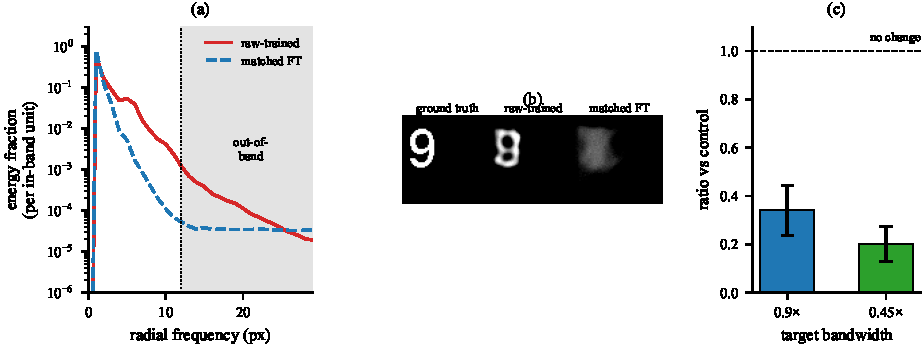
\includegraphics[width=0.95\textwidth]{figures/fig1_hero.pdf}
    \caption{Training-target bandwidth controls spectral fabrication. (a) Out-of-band energy is the reconstruction spectral energy outside the measured MTF support (shaded, vertical dotted line at the support radius); from an identical initialization, the raw-trained model keeps substantially more energy in this region (3$\times$ at the band edge) than the model fine-tuned against bandwidth-matched targets. (b) Reconstructions: the bandwidth-matched model suppresses out-of-band fabrication at the cost of visibly smoother (band-limited) output, which is the correct behavior under the measured information support; the raw-trained model restores sharper structure partly by inventing out-of-band content. (c) Suppression ratio of fine-tuned to compute-matched control out-of-band energy across both architectures and all seeds. Out-of-band energy is a fabrication proxy, not a perceptual metric.}
    \label{fig:hero}
\end{figure*}

% === Fig 2: paired control (single column) ===
\begin{figure}[t]
    \centering
    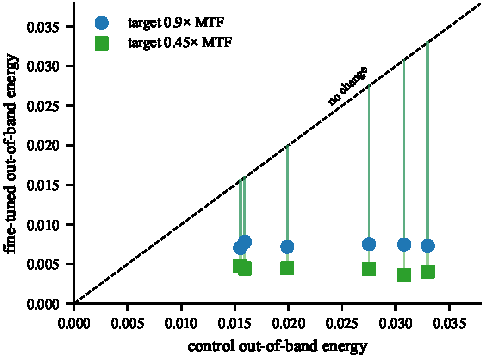
\includegraphics[width=0.48\textwidth]{figures/fig2_paired_control.pdf}
    \caption{Paired fine-tune versus compute-matched control (identical initialization; equal extra optimization). Each segment connects a unit's control value (on the no-change line) to its fine-tuned value. Matched-target ratio $0.34\pm0.11$ and half-target $0.20\pm0.08$; all 6/6 units reduce (one-sided sign test $p\approx0.016$).}
    \label{fig:paired}
\end{figure}

% === Fig 3: capacity (single column) ===
\begin{figure}[t]
    \centering
    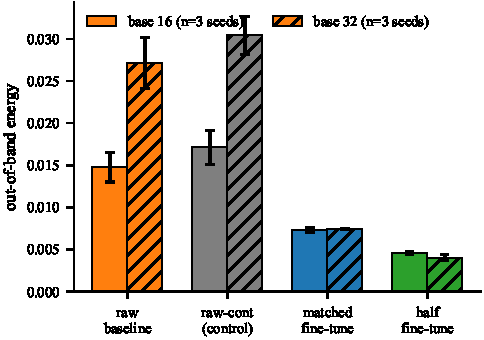
\includegraphics[width=0.48\textwidth]{figures/fig3_capacity.pdf}
    \caption{Out-of-band energy by arm for the two tested capacities. In the two tested capacities, the larger network fabricates more in the raw-baseline and control arms and admits stronger suppression under bandwidth-matched fine-tuning; described as an observed trend, not a scaling law. Error bars: std over 3 seeds.}
    \label{fig:capacity}
\end{figure}

% === Fig 4: trade-off (single column) ===
\begin{figure}[t]
    \centering
    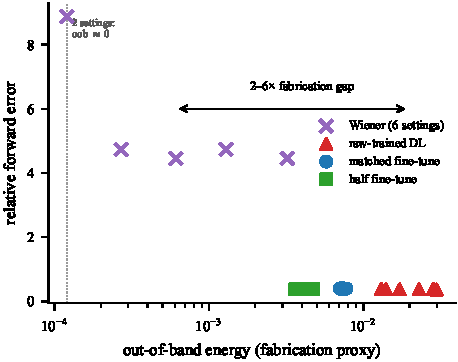
\includegraphics[width=0.48\textwidth]{figures/fig4_tradeoff.pdf}
    \caption{Fabrication versus forward fidelity. Wiener reconstructions (6 regularization/support settings) constrain out-of-band energy below the raw-target and matched arms in every cell (the half-bandwidth arm approaches the Wiener range) but operate at a roughly $1.4\times$ (${\sim}40\%$) worse relative forward error --- the learned arms therefore occupy a distinct operating point rather than dominating. Two Wiener settings with negligible out-of-band energy are drawn at the axis floor.}
    \label{fig:tradeoff}
\end{figure}

% === Fig 5: robustness (double column) ===
\begin{figure*}[t]
    \centering
    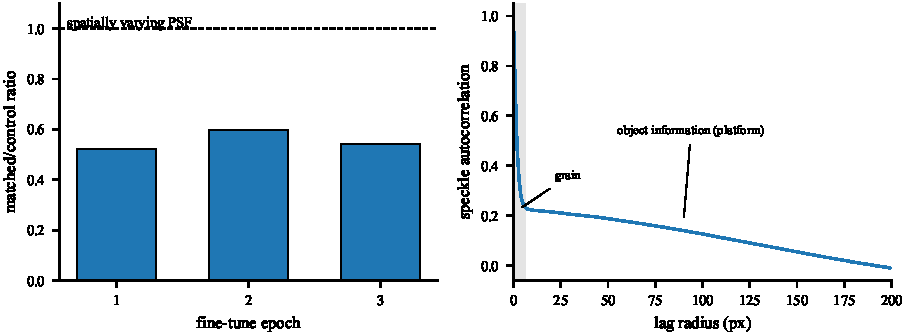
\includegraphics[width=0.92\textwidth]{figures/fig5_robustness.pdf}
    \caption{Left: the matched/control out-of-band ratio under a position-dependent (spatially varying PSF) forward operator remains stable across fine-tune epochs --- the suppression effect does not rely on shift-invariance. Right: measured speckle autocorrelation from the public experimental dataset (DSC): a sub-pixel grain peak superposed on a wide platform that carries object information out to $\sim$190\,px lag --- the real-data structure our protocol targets; quantitative real-data reconstruction is left to future work (see text).}
    \label{fig:robustness}
\end{figure*}

% === Table 1 ===
\begin{table}[t]
\centering
\small
\caption{Out-of-band energy (fabrication proxy) and band-limited PSNR across arms; mean$\pm$std over 6 units (2 architectures $\times$ 3 seeds). The paired block reports fine-tune-to-control ratios within units.}
\label{tab:main}
\begin{tabular}{lcc}
\toprule
Arm & Out-of-band energy & PSNR (dB) \\
\midrule
Raw baseline (20 ep) & $0.0210 \pm 0.0073$ & $16.5 \pm 0.4$ \\
Bandwidth-matched baseline (20 ep) & $0.0066 \pm 0.0006$ & $31.7 \pm 1.3$ \\
Half-bandwidth baseline (20 ep) & $0.0036 \pm 0.0004$ & $22.1 \pm 1.2$ \\
Raw-continued control (+4 ep) & $0.0238 \pm 0.0077$ & $16.4 \pm 0.5$ \\
Matched fine-tune (4 ep) & $0.0074 \pm 0.0003$ & $29.8 \pm 0.9$ \\
Half fine-tune (4 ep) & $0.0043 \pm 0.0004$ & $21.8 \pm 0.2$ \\
\midrule
\multicolumn{3}{l}{Paired (fine-tune vs.\ control, within unit)} \\
Matched fine-tune ratio & $0.34 \pm 0.11$ & reduced 6/6 \\
Half fine-tune ratio & $0.20 \pm 0.08$ & reduced 6/6 \\
\bottomrule
\end{tabular}
\end{table}



\subsection{Baselines and the reference-dependence of fidelity}
\label{sec:baselines}

Table~\ref{tab:main} summarizes all arms. The three from-scratch baselines (20 epochs each) show the expected monotone ordering in fabrication: the raw-target model reaches $\oob = 0.0210 \pm 0.0073$, the bandwidth-matched model $0.0066 \pm 0.0006$ ($3.2\times$ lower), and the half-bandwidth model $0.0036 \pm 0.0004$ ($5.9\times$ lower). The band-limited PSNR ordering, however, inverts: the matched model scores $31.7$~dB, well above the raw model's $16.5$~dB and the half model's $22.1$~dB. The inversion is not paradoxical: PSNR is computed against a reference low-pass filtered at the matched bandwidth, and the raw model's out-of-band energy is penalized twice under that reference---once as fabrication, and once because the reference contains no such energy to match. This is why the protocol reports band-limited PSNR as a secondary, reference-dependent quantity and uses the no-reference forward-consistency endpoint for the causal comparison: the ranking of models under a reference-based fidelity metric depends on the bandwidth of the reference, and a benchmark result quoted without its reference bandwidth is under-specified.

\subsection{The causal intervention: fine-tuning versus compute-matched control}
\label{sec:main-control}

Fig.~\ref{fig:paired} shows the central result. Each segment connects one unit's control value (the continuation arm, on the no-change line) to the same unit's fine-tuned value, so every segment is a paired within-unit comparison under identical initialization and identical additional optimization. The matched-target fine-tune reduces out-of-band energy to a ratio of $0.34 \pm 0.11$ of its control, and the half-target fine-tune to $0.20 \pm 0.08$; all six units reduce in both settings (one-sided sign test $p \approx 0.016$), and the pre-registered criterion (ratio $< 0.8$) is met with margin. The model trained from scratch on matched targets reaches the same low fabrication level, while the compute-matched control moves in the \emph{opposite} direction: four additional epochs on the raw target increase fabrication from $0.0210$ to $0.0238$ on average across units (about $13\%$); the continuation is not a passive arm that merely freezes.

The no-reference endpoint rules out the trivial explanation that suppression is achieved by degrading the reconstruction into smoothness. The relative forward consistency of the matched fine-tune changes by a mean paired difference of $+0.026$ on a $0.36$--$0.40$ baseline---a small relative increase that bounds the fidelity cost of the suppression at roughly 7\% of the baseline forward error (the half-bandwidth \emph{baseline} sits at a distinct operating point, up to $0.47$, and is excluded from this comparison range). Fabrication suppression and measurement agreement are therefore close to unchanged rather than traded against each other, and the half-target arm moves by only $+0.006$. Fig.~\ref{fig:hero}(b) shows the qualitative behavior behind these numbers: at the matched bandwidth, the fine-tuned reconstruction is visibly smoother than the raw model's, and that smoothness is the correct band-limited behavior---the raw model's extra apparent structure is largely content the measurement cannot certify.

\subsection{Fabrication grows with capacity}
\label{sec:capacity}

Fig.~\ref{fig:capacity} splits the arms by network width. In the two tested capacities, the larger network (base 32) exhibits higher raw fabrication: $0.027$ versus $0.015$ in the raw baseline, and $0.030$ versus $0.017$ in the control. Suppression is correspondingly stronger for the larger network: the matched fine-tune ratio is $0.25$ for base 32 versus $0.44$ for base 16. These contrasts are point estimates over three seeds per width (per-arm variability in Table~\ref{tab:main}). Read together with Sec.~\ref{sec:wiener}, the pattern is consistent with the informal hypothesis that extra capacity is spent, in part, on fabricating content beyond the measurement---and that bandwidth-matched targets reclaim that capacity for in-support reconstruction. We state this as an observed trend across the two tested widths, not as a scaling law; three or more capacity points would be required to establish the functional form.

\subsection{The Wiener anchor: a trade-off, not a defeat}
\label{sec:wiener}

How much fabrication is avoidable in principle? A Wiener filter with the known PSF is the optimal linear reconstruction under the protocol's noise model, and it cannot fabricate out-of-band content: its output energy outside the measured support is bounded by its regularization. Across a grid of six regularization/support settings, the Wiener reconstruction's out-of-band energy stays in $0.0003$--$0.0032$---$2$--$6\times$ below the raw-target and matched arms in every cell, while the half-bandwidth arm approaches the Wiener range (the worst Wiener cell is within ${\sim}1.1\times$ of the half arm's mean); two settings drive it to numerical zero (Fig.~\ref{fig:tradeoff}). The same grid, however, shows the price: evaluated under the same relative-forward-error definition with an optimal scalar rescaling of its output (a fair comparison, since a raw Wiener estimate is not amplitude-calibrated), Wiener's relative forward error is $0.52$--$0.55$, versus $0.36$--$0.40$ for the learned arms---roughly $40\%$ higher. The linear baseline is spectrally conservative because it remains under-fitted: it fails to re-explain its own measurement by about $1.4\times$ more than the learned arms. The learned arms therefore occupy a distinct operating point in the (fabrication, forward-fidelity) plane rather than dominating or being dominated. The bandwidth-matched fine-tune moves a learned model toward, but not to, the linear regime---the honest summary of the trade-off is that fabrication can be controlled by at least $3\times$ at a fidelity cost bounded at about $7\%$ of the baseline forward error, not that it can be eliminated for free.

\subsection{Robustness to a position-dependent forward operator}
\label{sec:svpsf}

The protocol above assumes a shift-invariant PSF. Real scattering systems violate this: the PSF varies across the field, and the memory-effect range is finite. To test whether the suppression effect rides on the shift-invariance idealization, we replace the single PSF with a position-dependent operator: four independently seeded PSFs blended by feathered quadrant masks, so the forward operator changes with position while its local statistics stay matched. Under this operator, retraining the same arms reproduces the effect: the matched-to-control out-of-band ratio is $0.52$, $0.60$, $0.54$ at one, two, and four fine-tune epochs---stable across optimization length and clearly separated from the no-change line (Fig.~\ref{fig:robustness}, left). These levels come from a single-seed robustness configuration with a different forward operator and are therefore not directly comparable to the multi-seed main result of Sec.~\ref{sec:main-control}; the quantity this experiment establishes is the \emph{stability and sign} of the suppression under a broken shift-invariance assumption. A companion fine-tune-length sweep under the shift-invariant protocol shows the same stability ($0.52$, $0.49$, $0.50$), which rules out a transient-optimization explanation for the suppression. The mechanism therefore does not require exact shift invariance.

\subsection{Negative control: no class boundary in transfer loss}
\label{sec:negative}

The field's standard training protocol is defined over ``same-class'' diffusers \cite{li2018deep}. If cross-diffuser transfer loss were governed by a genuine class boundary, protocol design could target class membership; if not, the label is a convenience and quantitative statistics---reported distance, measured bandwidth---should replace it. We trained twelve decoders on twelve synthetic diffusers arranged as an orthogonal grid over three factors (pupil radius, phase-height distribution, phase-spectrum smoothness), evaluated the full $12\times12$ transfer matrix on identical test objects, and fitted each of three statistical distances (height-map Wasserstein, speckle power-spectrum Jensen--Shannon, patch-level MMD) against the paired transfer losses. Under all three metrics, a segmented (changepoint) fit fails to beat a smooth monotone fit by the model-selection criterion ($\Delta\text{BIC} = \text{BIC}_{\text{segmented}} - \text{BIC}_{\text{smooth}} = -1.4, +5.6, +3.3$ respectively; positive values favor the smooth fit, and none clears the $-10$ threshold that would favor a changepoint), and permutation tests put the changepoint's apparent gains inside the null distribution ($p = 0.08, 0.91, 0.41$). Two of the twelve decoders (strong-scattering binary-phase diffusers) converge to partially object-independent solutions for out-of-family inputs; we disclose this and verify that the conclusion is insensitive to it---excluding both affected decoders leaves every metric inside the null distribution ($\Delta$BIC ranges from $-1.1$ to $+0.6$, permutation $p = 0.11$--$0.18$). Transfer loss varies smoothly with distance; there is no boundary to find. One further caution: the largest observed losses (up to $15.0$~dB) occur where a single distance is smallest but another factor differs---each distance is blind to the factors it does not measure---so a scalar law would need the joint distance, and we report the negative control as evidence for protocol-level reporting rather than as a claimed law. The full matrix and fit details are deferred to the supplementary material.

\section{Real-Data Assessment}
\label{sec:realdata}

The protocol above is simulation-based, and its central quantity---out-of-band energy---is defined against a known forward operator. Assessing how far the protocol extends to real measurements requires a system whose information support can be measured directly. We used a public experimental speckle dataset (measured through diffusers, paired ground-truth digits; 240 of its files sampled) and report what the protocol can and cannot deliver on it.

\paragraph{What is measurable.} The speckle power spectrum yields the system's information support: the grain full-width at half-maximum is $1.93$~px, corresponding to an MTF-support radius of roughly 52\% of Nyquist. The speckle intensity autocorrelation (Fig.~\ref{fig:robustness}, right) decomposes into a narrow grain peak (FWHM $\approx 1.9$~px) superposed on a wide platform extending to $\sim$$191$~px lag---the platform is the object information that speckle-correlation reconstruction classically exploits, and its stability across the dataset ($191 \pm 1.3$~px) identifies it as a system-level memory-effect/field-of-view quantity rather than an object property. A paired signal is detectable at the autocorrelation level: same-object matches separate from mismatched pairs (2D autocorrelation NCC $0.60$ versus $0.50$, Welch $t = 3.2$ over 15 pairs), so the dataset supports paired analysis. Pixel-level speckle--ground-truth correlations, by contrast, are too weakly separated to serve as a pairing statistic (means within ${\sim}0.01$ of each other over 20 pairs), which is why the paired analysis above operates at the correlation-structure level.

\paragraph{What is not yet available.} A quantitative bandwidth-protocol statement on this data---the real-data analogue of Sec.~\ref{sec:main-control}---requires a calibrated forward operator, and we did not obtain one under a minimal protocol. Three registration approaches failed systematically: (i) a cross-spectral transfer-function estimate degenerates, consistent with the recorded mapping not being a well-conditioned shift-invariant convolution at the object's recorded scale (the reliable structure lives in the autocorrelation domain, per the Siegert relation); (ii) radial autocorrelation matching is confounded because the system-level platform dominates the profile while the object's autocorrelation is not radially symmetric; (iii) two-dimensional autocorrelation scale matching produced a chaotic scale estimate (coefficient of variation $1.02$, values piling at both search boundaries). The failure pattern identifies the obstacle: this dataset was constructed so that the object-to-speckle mapping is learned end-to-end precisely because it is not analytically parsimonious, and our minimal registration protocol could not recover the operator from paired samples alone. Applying a bandwidth protocol to such data therefore requires a dedicated forward-calibration stage---either analytic or learned---which is a research task in its own right and is not a preprocessing detail. We report this boundary condition explicitly: the real-data section of this paper quantifies the environment (support, correlation structure, pairing statistics) and states plainly that the causal claim is established in simulation.

\section{Discussion, Limitations, and Conclusion}
\label{sec:discussion}

\subsection{What the evidence establishes}

Three findings form the paper's causal spine. First, the bandwidth of the training target is a genuine causal control of spectral fabrication, not a correlate: changing only that choice, from an identical initialization and with identical additional optimization, cuts measured out-of-band energy to about one third of the matched control, 6/6, with the no-reference forward-consistency endpoint ruling out a smoothness-degradation explanation. Second, fabrication is not free of capacity: in the two tested widths it is the larger network that fabricates more, and that admits stronger suppression---capacity that bandwidth-matched targets redirect rather than remove. Third, the linear Wiener baseline shows what the trade-off landscape looks like from the outside: fabrication can be pushed below the learned range, but only by accepting a roughly $1.4\times$ (about $40\%$) worse forward fit. The practical statement for practitioners is deliberately modest and operational: audit your training target's bandwidth against your system's measured support before auditing your network.

\subsection{Limitations}

The causal claims are established under simulated protocols: a shift-invariant speckle model (plus the position-dependent robustness variant), a single noise model, $64\times64$ images, two network widths, three seeds, and digit objects. Out-of-band energy is a fabrication proxy anchored to a measured physical support, not a perceptual or semantic metric. The capacity result covers two widths and is stated as an observed trend. The distance-law negative control relies on three metric choices and twelve diffuser families. Real-data evidence is preliminary: system parameters and pairing statistics are quantified, but no quantitative real-data reconstruction claim is made, and the failed registration approaches delimit rather than solve the forward-calibration problem. The fine-tune comparison, though compute-matched, involves a single fine-tune length per setting in the main arm (the length sweep in Sec.~\ref{sec:svpsf} addresses stability, not exhaustiveness).

\subsection{Future work}

Two directions follow directly. (i) \emph{Objects beyond digits and one real forward-calibration}: extending objects to natural-image statistics and building the forward-calibration stage that the real-data section identifies would let the protocol cross from simulation to measured systems. (ii) \emph{Bandwidth as a deployment dial}: the intervention costs nothing and is compatible with any training pipeline; characterizing it under temporal integration regimes and multi-wavelength acquisition would test whether measured support should be treated as a first-class hyperparameter of learned reconstruction.

\subsection{Conclusion}

We isolated the bandwidth of the training target as a causal, compute-matched control of spectral fabrication in learned speckle reconstruction. Bandwidth-matched fine-tuning reduces out-of-band fabrication to $0.34 \pm 0.11$ (matched) and $0.20 \pm 0.08$ (half) of an identically optimized control (6/6 units, sign test $p \approx 0.016$) while leaving the no-reference forward-consistency endpoint nearly unchanged ($+0.026$ on a $0.36$--$0.40$ baseline); raw fabrication and suppression strength both grow with capacity in the tested range; and a Wiener anchor shows the control operates within a trade-off landscape where the spectrally conservative linear baseline remains under-fitted by about $40\%$ in relative forward error. A cross-diffuser analysis finds no class boundary, and a real-data assessment quantifies system parameters while marking the forward-calibration requirement as the boundary of the simulation-based claim. Fabrication in learned speckle imaging is, in part, a choice made in the training data---and it can therefore be audited, controlled, and reported as one.


\section*{Acknowledgment}
[Funding acknowledgment to be completed (grant agency, project number, or a statement that no external funding was received).]

\bibliographystyle{IEEEtran}
\bibliography{references}

\end{document}
